% !TEX root = Main.tex
\documentclass[Main]{subfiles}

\begin{document}
\section{Normalized Appearance and Shape Method Using SVM} % (fold)
	\label{sec:normalized_appearance_and_shape_method_using_svm}
	In this section I describe how I tried to reproduce the results of \cite{Lucey2011} by implementing my own algorithm for extracting data and training a linear Support Vector Machine (SVM) using LIBSVM \cite{CC01a}.

	The data extracted from the database and used in the experiments are normalized shape and shape normalized appearance (described in greater detail in Section \ref{sub:data_pre_processing_and_feature_extraction} below).
	Two experiments will be done with these data.
	One will focus on detecting the presence of FACS Action Units relevant to PSPI model described in Section \ref{ssub:pain_score}.
	The other will focus only on the detection of pain.
	Both will experiments will tested using the shape data alone and with shape and appearance data combined.

	% Method

		% Procustes alignment of faces
		% Delauney triangulation of mean shape
		% New triangulation of aligned faces
		% Affine warp to mean shape
		% Extract and vectorize appearance
		% 

		
	% My implementation
	% My Results
	% Discuss, compare and reference results
		% Strong points
		% Shortcomings

	\subsection{Data pre-processing and Feature Extraction} % (fold)
		\label{sub:data_pre_processing_and_feature_extraction}

		\subsubsection{Shape Data} % (fold)
			\label{ssub:shape_data}
			The raw shape data consists of \texttt{.txt}-file for each frame with two columns of (x,y) pixel coordinates, 66 points in total each for a specific facial landmark.
			\fxnote{insert image of facial landmarks, possibly numbered} 
			These combined make a mask of the facial shape.
			They are however centered in the corner of the image and shifted, scaled and rotated arbitrarily form subject to subject and from frame to frame because of movement.

			\paragraph{Procrustes Alignment} % (fold)
				\label{par:procrustes_alignment}
				In order to use the shape data they need to be shifted to a zero mean reference and be normalized with regard to size and rotation, without affecting shape.
				For this, Procrustes alignment is just what is needed.
				Procrustes alignments works by aligning sets of points to a common reference (either given, or taken as the mean of the set to be aligned) by a rigid transformation ie. translation, rotation and scale.

				In my project I do this iteratively and by using MATLABs build in \texttt{procrustes} function, like so:
				\begin{enumerate}

					\item
					For each shape $\textbf{S}_i$ subtract the mean of all points in $\textbf{S}_i$.

					\item
					Calculate mean shape $\textbf{Z}_0$, by taking the mean over all shapes $\textbf{S}_i$ for each point $\textbf{S}_{i,j}$.

					\item
					\label{enum:goto}
					Align all shapes $\textbf{S}_i$ to $\textbf{Z}_0$ using \texttt{procrustes} to get the aligned shapes $\textbf{Z}_i$.

					\item
					Calculate the new mean shape $\textbf{Z}_0$ over all shapes $\textbf{Z}_i$ for each point $\textbf{Z}_{i,j}$.

					\item
					Repeat from step \ref{enum:goto} for as many times as is needed. 
					A typical stopping criteria is when $\textbf{Z}_0$ stops changing significantly.

				\end{enumerate}
				Two iterations will typically suffice and is therefore what is used in this project.

				The result is what \cite{Lucey2011} and \cite{Ashraf2009} call the  \emph{similarity normalized shape} or \textbf{S-PTS}.
				This is a vector of x and y-coordinates $\textbf{s}_n$.

				% paragraph procrustes_alignment (end)

			% subsubsection shape_data (end)


		\subsubsection{Appearance Data} % (fold)
			\label{ssub:appearance_data}
			In order to be able to compare and classify the appearance of different subjects with an SVM, the image data from each frame has to be normalized.
			The representation of image data need to be invariant to several factors:
			\begin{itemize}
				\item
				The subject's face can be in different parts of the image frame.

				\item
				Subjects' faces can vary in size, both from physical size and from proximity to the camera.

				\item
				The subject's face can be rotated/tilted sideways as a result of posture and moving the arm.

				\item
				The background is not uniform and varies from sequence to sequence.

				\item
				The general shape of a subjects face varies from subject to subject.

			\end{itemize}

			The goal is to sample to image at a set amount of points that maps to a fixed pixel mask, called \emph{objectPixels}.
			This way the appearance is represented as a vector of pixel intensities, that maps to a common face shape with the background excluded.
			
			Two strategies exist for doing this.
			One \cite{Ashraf2009} calls  \emph{similarity normalized appearance} or \textbf{S-APP}.
			Here the pixels are sampled inside the shape bounded by the facial landmarks and transformed rigidly according to the Procrustes alignment described in Section \ref{par:procrustes_alignment} above.
			This method seems to preserve most variation caused by facial actions but also results in more spatial variation of the position of features in the image representation, called $\textbf{a}_n$.

			Another strategy what \cite{Lucey2011} and \cite{Ashraf2009} call the \emph{canonical appearance} or \textbf{C-APP}.
			This method samples the intensities inside the shape bounded by the facial landmarks and warps their position in a non-rigid fashion, to match the mean shape $\textbf{Z}_0$.
			This method removes more of the spatial variation of the position of features in the resulting image representation, $\textbf{a}_0$

			\begin{figure}[H]
				\begin{center}
					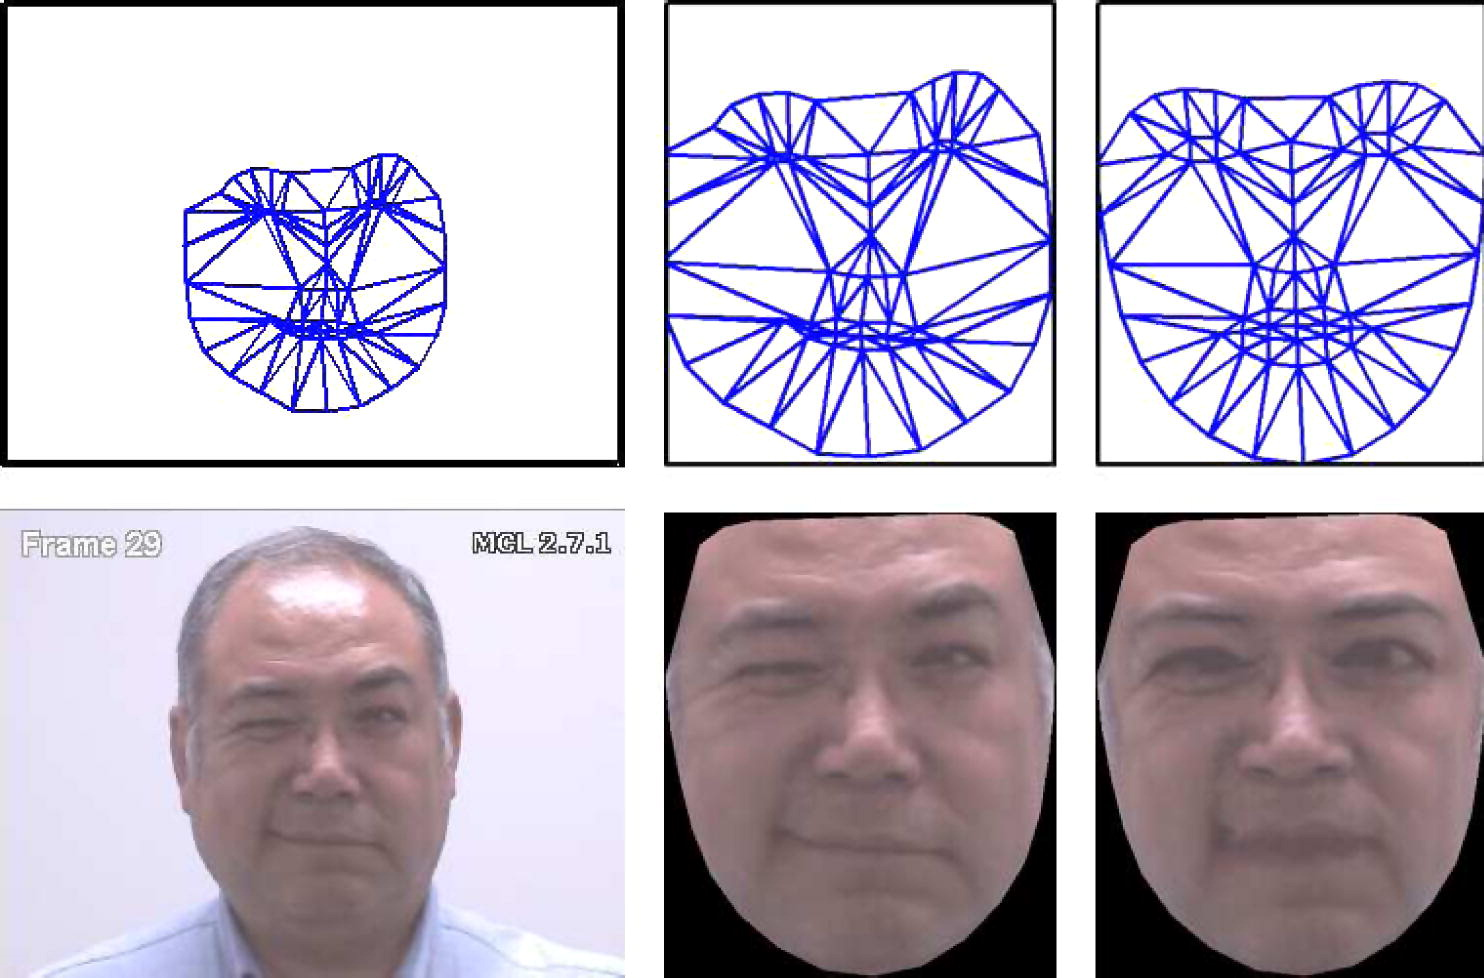
\includegraphics[width=0.7\textwidth]{C-APP_Example}
				\end{center}
				\caption{
					Example of image representations.
					Top row: Left, triangulation of raw landmarks. Middle, Procrustes aligned shape. Right, mean shape.
					Bottom row: Left, raw image. Middle, \textbf{S-APP}. Right, \textbf{C-APP}.
					Figure taken from \cite{Ashraf2009}.
					}
				\label{fig:app_strategies}
			\end{figure}
			
			A comparison of the two strategies is shown in Figure \ref{fig:app_strategies}.
			As \cite{Ashraf2009} rightly notes, it would seem that \textbf{C-APP} removes too much variation, eg. in the case of an eye closure as shown in Figure \ref{fig:app_strategies}.
			The case is though that \textbf{C-APP} preserves the most important part of this action, because the wrinkles around the eye is still very clear.
			These serve to distinguish between a \emph{twitch} as a result of pain and a regular blink, which does not result in these wrinkles.
			This distinction is a common cause for false positives in a pain recognition system.
			Further, the supposed lost information is conserved if the shape data and appearance is used together.

			In this project the \textbf{C-APP} representation is used.

			\paragraph{Implementing Image Warping} % (fold)
				\label{par:implementing_image_warping}
				The non-rigid warp of the facial appearance to the mean shape is done with at piecewise affine transformation.
				This means segmenting the face into triangles and the for each triangle warping the pixels inside to the corresponding triangle in the reference mean shape.
				The procedure is implemented as follows:
				\footnote{
					This is a general description of the implemented method. 
					For full MATLAB implementation see files \texttt{WarpImagesToMeanBatch.m} and \texttt{warpAppToMeanShape.m} in Appendix {\ref{sec:code}}
					}
				\begin{enumerate}
					\item
					The landmark points of the mean face shape needs to be put into a graph that connects all vertices into triangles without overlapping edges.
					There exists many solutions for this problem, but by making a Delauney triangulation, one can find the single solution that maximizes the smallest angle in all the triangles.
					This solution tends to avoid \emph{skinny} triangles and is a good fit for this application.

					The Delauney triangulation is made using MATALB's \texttt{delaunayTriangulation} function.
					It takes a set of points as input and returns a \emph{triangulation} object, which contain information about which vertices are connected in triangles (also called a \emph{Connectivity List}), and methods to determine in which triangle a certain point is inside.

					\item
					\emph{objectPixels} is determined by evaluating which pixel position is not inside any triangle of the Delauney triangulation of the mean shape.
					This results in a matrix of xy-coordinates, one row for each pixel.

					\item
					For each frame a new \emph{triangulation} object is then created using the connectivity list of the Delauney triangulation of the mean shape and the facial landmark points.
					This new triangulation is not an optimal Delauney triangulation.
					Instead it is a triangulation of the point in the frame where the triangle connections correspond to that of the Delauney triangulation of the mean shape.

					







				\end{enumerate}


				
				% paragraph implementing_image_warping (end)

			\paragraph{Delauney Triangulation} % (fold)
				\label{par:delauney_triangulation}
				
				% paragraph delauney_triangulation (end)

			\paragraph{Piecewise Affine Warp} % (fold)
				\label{par:piecewise_affine_warp}
				
				% paragraph piecewise_affine_warp (end)




				\subparagraph{subparagraph name} % (fold)
				\label{subp:subparagraph_name}
				
				lalala
				% subparagraph subparagraph_name (end)


			% subsubsection appearance_data (end)

		\subsubsection{Combining Data} % (fold)
			\label{ssub:combining_data}

			% Vectorization
			
			% subsubsection combining_data (end)
		
		% subsection data_pre_processing_and_feature_extraction (end)


	\subsection{Experiment 1: Recognizing FACS Action Units} % (fold)
		\label{sub:experiment_1_recognizing_facs_action_units}
		
		% subsection experiment_1_recognizing_facs_action_units (end)


	\subsection{Experiment 2: Detecting Pain in faces} % (fold)
		\label{sub:experiment_2_detecting_pain_in_faces}
		
		% subsection experiment_2_detecting_pain_in_faces (end)


	\subsection{Discussion} % (fold)
		\label{sub:discussion}
		
		% subsection discussion (end)

	% section normalized_appearance_and_shape_method_using_svm (end)


\end{document}